\documentclass[11pt]{article}

\usepackage[margin=0.82in]{geometry}
\usepackage[T1]{fontenc}
\usepackage[utf8]{inputenc}
\usepackage{lmodern}
\usepackage{microtype}
\usepackage{amsmath,amssymb,mathtools}
\usepackage{booktabs,longtable,array,tabularx}
\usepackage[table]{xcolor}
\usepackage{enumitem}
\usepackage{hyperref}
\usepackage{tikz}
\usepackage{pgfplots}
\usepackage[most]{tcolorbox}
\usepackage{caption}
\usepackage{float}
\usepackage{fancyhdr}
\usepackage{titlesec}

\usetikzlibrary{arrows.meta,positioning,fit,calc,shapes.geometric,decorations.pathreplacing}
\pgfplotsset{compat=1.18}

\definecolor{navy}{RGB}{24,45,75}
\definecolor{ink}{RGB}{35,49,70}
\definecolor{slate}{RGB}{79,96,119}
\definecolor{fixedblue}{RGB}{59,130,246}
\definecolor{fixedpale}{RGB}{231,240,254}
\definecolor{observedgold}{RGB}{219,151,30}
\definecolor{observedpale}{RGB}{255,245,216}
\definecolor{unknownpurple}{RGB}{132,84,194}
\definecolor{unknownpale}{RGB}{241,233,252}
\definecolor{calcteal}{RGB}{17,146,137}
\definecolor{calcpale}{RGB}{222,245,242}
\definecolor{outputgreen}{RGB}{53,139,82}
\definecolor{outputpale}{RGB}{229,245,233}
\definecolor{coral}{RGB}{226,91,78}
\definecolor{coralpale}{RGB}{253,233,230}
\definecolor{lightgray}{RGB}{245,247,250}
\definecolor{midgray}{RGB}{215,223,232}

\hypersetup{
  colorlinks=true,
  linkcolor=calcteal,
  urlcolor=fixedblue!70!black,
  citecolor=unknownpurple,
  pdftitle={ShapeMix-ATAC One Step at a Time},
  pdfauthor={Andy Zhuang},
  pdfsubject={Progressive tutorial for the ShapeMix-ATAC Bayesian model},
  pdfkeywords={ShapeMix, ATAC-seq, Bayesian model, deconvolution, fragment length, MAP}
}

\setlength{\headheight}{14pt}
\setlength{\parindent}{0pt}
\setlength{\parskip}{0.43em}
\renewcommand{\arraystretch}{1.18}
\pagestyle{fancy}
\fancyhf{}
\lhead{ShapeMix-ATAC, one step at a time}
\rhead{Progressive model tutorial}
\cfoot{\thepage}

\titleformat{\section}{\Large\bfseries\color{navy}}{\thesection}{0.65em}{}
\titleformat{\subsection}{\large\bfseries\color{calcteal}}{\thesubsection}{0.65em}{}
\titleformat{\subsubsection}{\normalsize\bfseries\color{unknownpurple}}{\thesubsubsection}{0.65em}{}

\newcolumntype{L}[1]{>{\raggedright\arraybackslash}p{#1}}
\newcolumntype{C}[1]{>{\centering\arraybackslash}p{#1}}

\newcommand{\NB}{\operatorname{NegBinomial}}
\newcommand{\Mult}{\operatorname{Multinomial}}
\newcommand{\Gam}{\operatorname{Gamma}}
\newcommand{\Pois}{\operatorname{Poisson}}
\newcommand{\E}{\mathbb{E}}
\newcommand{\Var}{\operatorname{Var}}
\newcommand{\given}{\,|\,}
\newcommand{\fixedq}[1]{\textcolor{fixedblue!75!black}{#1}}
\newcommand{\obsq}[1]{\textcolor{observedgold!80!black}{#1}}
\newcommand{\unknownq}[1]{\textcolor{unknownpurple}{#1}}
\newcommand{\calcq}[1]{\textcolor{calcteal!85!black}{#1}}
\newcommand{\outputq}[1]{\textcolor{outputgreen!85!black}{#1}}

\newtcolorbox{bigidea}{
  colback=fixedpale,
  colframe=fixedblue!75!black,
  title=Main idea,
  fonttitle=\bfseries,
  breakable
}
\newtcolorbox{newvar}[1]{
  colback=lightgray,
  colframe=navy,
  title={New symbol: #1},
  fonttitle=\bfseries,
  breakable
}
\newtcolorbox{checkpoint}{
  colback=outputpale,
  colframe=outputgreen!80!black,
  title=Pause and check,
  fonttitle=\bfseries,
  breakable
}
\newtcolorbox{watchout}{
  colback=coralpale,
  colframe=coral,
  title=Important distinction,
  fonttitle=\bfseries,
  breakable
}
\newtcolorbox{translation}{
  colback=calcpale,
  colframe=calcteal,
  title=Say the equation in words,
  fonttitle=\bfseries,
  breakable
}
\newtcolorbox{worked}[1]{
  colback=observedpale,
  colframe=observedgold,
  title=#1,
  fonttitle=\bfseries,
  breakable
}
\newtcolorbox{advanced}[1]{
  colback=white,
  colframe=slate,
  title={Advanced detail: #1},
  fonttitle=\bfseries,
  breakable
}

\begin{document}
\hypersetup{pageanchor=false}

\begin{titlepage}
\centering
\vspace*{0.25in}
{\Huge\bfseries\color{navy} ShapeMix-ATAC, One Step at a Time\par}
\vspace{0.16in}
{\LARGE\color{calcteal} Start with one number; end with the full Bayesian model\par}
\vspace{0.22in}
{\large A progressive tutorial with one running example and a new-symbol card for every new variable\par}

\vspace{0.50in}
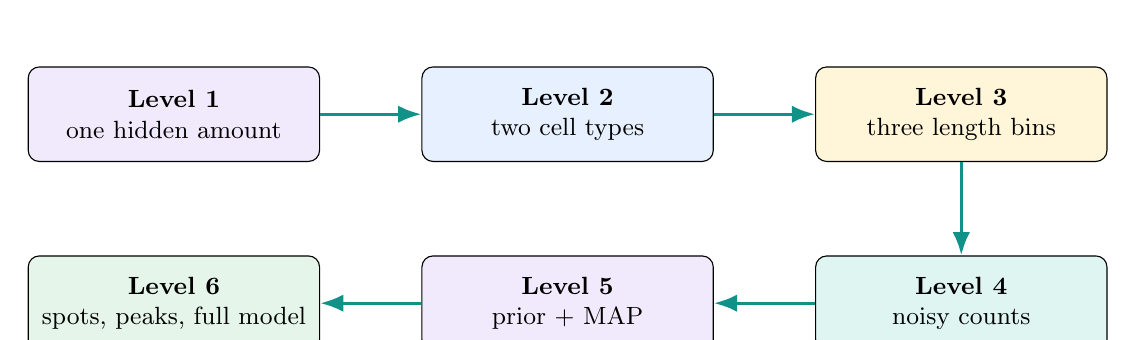
\begin{tikzpicture}[>=Latex,every node/.style={align=center,font=\small}]
  \node[draw,rounded corners,fill=unknownpale,minimum width=3.7cm,minimum height=1.2cm] (l1) at (0,1.4)
    {\textbf{Level 1}\\one hidden amount};
  \node[draw,rounded corners,fill=fixedpale,minimum width=3.7cm,minimum height=1.2cm] (l2) at (5.0,1.4)
    {\textbf{Level 2}\\two cell types};
  \node[draw,rounded corners,fill=observedpale,minimum width=3.7cm,minimum height=1.2cm] (l3) at (10.0,1.4)
    {\textbf{Level 3}\\three length bins};
  \node[draw,rounded corners,fill=calcpale,minimum width=3.7cm,minimum height=1.2cm] (l4) at (10.0,-1.0)
    {\textbf{Level 4}\\noisy counts};
  \node[draw,rounded corners,fill=unknownpale,minimum width=3.7cm,minimum height=1.2cm] (l5) at (5.0,-1.0)
    {\textbf{Level 5}\\prior + MAP};
  \node[draw,rounded corners,fill=outputpale,minimum width=3.7cm,minimum height=1.2cm] (l6) at (0,-1.0)
    {\textbf{Level 6}\\spots, peaks, full model};
  \draw[->,very thick,calcteal] (l1) -- (l2);
  \draw[->,very thick,calcteal] (l2) -- (l3);
  \draw[->,very thick,calcteal] (l3.south) -- (l4.north);
  \draw[->,very thick,calcteal] (l4) -- (l5);
  \draw[->,very thick,calcteal] (l5) -- (l6);
\end{tikzpicture}

\vfill
\begin{bigidea}
The tutorial keeps the same example all the way through: one spot contains a
T-cell-like amount of \(1.5\) effective units and a B-cell-like amount of \(0.5\)
units. Together they predict \(24\) cut sites, divided as \(10\) short-parent,
\(8\) mono-parent, and \(6\) long-parent cut sites. We will not show the indexed
version of the model until every part of this example makes sense.
\end{bigidea}

\vfill
{\large Progressive rewrite, version 2.0\par}
{\large August 27, 2026\par}
\end{titlepage}

\hypersetup{pageanchor=true}
\pagenumbering{roman}
\setcounter{tocdepth}{1}
\tableofcontents
\newpage
\pagenumbering{arabic}

\section{How to read this tutorial}

The old way to present this model is to display the complete tensor equation and
then define its symbols. This tutorial does the reverse:

\begin{enumerate}[leftmargin=2em]
  \item explain a scientific object in ordinary language;
  \item calculate it using the running numbers;
  \item give it a short mathematical name; and
  \item only later attach indices for many spots, peaks, bins, and cell types.
\end{enumerate}

The colors show each quantity's job:

\begin{center}
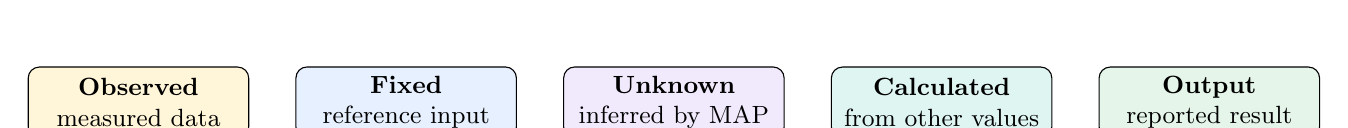
\begin{tikzpicture}[every node/.style={font=\small,align=center}]
  \node[draw,rounded corners,fill=observedpale,minimum width=2.8cm,minimum height=0.9cm] at (0,0)
    {\textbf{Observed}\\measured data};
  \node[draw,rounded corners,fill=fixedpale,minimum width=2.8cm,minimum height=0.9cm] at (3.4,0)
    {\textbf{Fixed}\\reference input};
  \node[draw,rounded corners,fill=unknownpale,minimum width=2.8cm,minimum height=0.9cm] at (6.8,0)
    {\textbf{Unknown}\\inferred by MAP};
  \node[draw,rounded corners,fill=calcpale,minimum width=2.8cm,minimum height=0.9cm] at (10.2,0)
    {\textbf{Calculated}\\from other values};
  \node[draw,rounded corners,fill=outputpale,minimum width=2.8cm,minimum height=0.9cm] at (13.6,0)
    {\textbf{Output}\\reported result};
\end{tikzpicture}
\end{center}

\begin{watchout}
The normative executable definition remains
\texttt{docs/ShapeMix/model\_specification.md}. This document explains that model;
it does not replace the specification.
\end{watchout}

\section{Before equations: what goes in and what comes out?}

\subsection{The output is a mixture, not a cell-type label}

For each spatial spot, ShapeMix reports one row of estimated cell-type
proportions. For example:

\begin{center}
\begin{tabular}{L{0.22\linewidth}C{0.20\linewidth}C{0.20\linewidth}C{0.20\linewidth}}
\toprule
Spot & T cell & B cell & Monocyte \\
\midrule
spot 1 & 0.65 & 0.25 & 0.10 \\
\bottomrule
\end{tabular}
\end{center}

The row sums to one. It means that normalizing the MAP abundance estimate gives
approximately \(65\%\) T-cell-like, \(25\%\) B-cell-like, and \(10\%\)
monocyte-like composition.

\begin{watchout}
This row is not a confidence distribution. The current ShapeMix MVP reports one
MAP point estimate. It does not report credible intervals, confidence intervals,
or posterior samples.
\end{watchout}

\subsection{The input counts cut sites}

One deduplicated ATAC fragment has two Tn5 cut sites, one at each end. ShapeMix
counts the cut sites that fall in selected peaks and labels each cut by the length
of its parent fragment.

\begin{figure}[H]
\centering
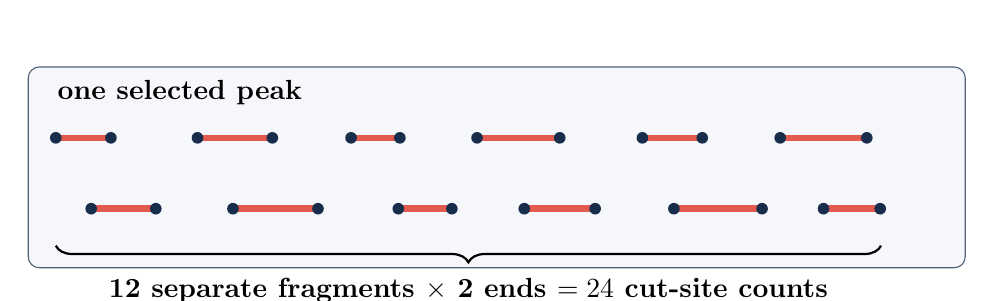
\begin{tikzpicture}[x=1cm,y=1cm]
  \draw[rounded corners,fill=lightgray,draw=slate] (-0.35,-1.2) rectangle (11.55,1.35);
  \node[anchor=west,font=\bfseries] at (-0.1,1.03) {one selected peak};
  \foreach \x/\y/\len in {
    0/0.45/0.70,1.8/0.45/0.95,3.75/0.45/0.62,5.35/0.45/1.05,7.45/0.45/0.76,9.2/0.45/1.10,
    0.45/-0.45/0.82,2.25/-0.45/1.08,4.35/-0.45/0.68,5.95/-0.45/0.90,7.85/-0.45/1.12,9.75/-0.45/0.72
  } {
    \draw[line width=2.4pt,coral] (\x,\y) -- ++(\len,0);
    \fill[navy] (\x,\y) circle (2.1pt);
    \fill[navy] ({\x+\len},\y) circle (2.1pt);
  }
  \draw[decorate,decoration={brace,mirror,amplitude=6pt},thick]
    (0,-0.92) -- (10.48,-0.92)
    node[midway,below=8pt,font=\bfseries] {12 separate fragments \(\times\) 2 ends \(=24\) cut-site counts};
\end{tikzpicture}
\caption{The fragment bars are separate observations. The two dark endpoints of each bar are the primary count units.}
\end{figure}

If both endpoints of all 12 fragments land in this peak, the peak total is 24.
In real data a fragment can contribute zero, one, or two selected-peak cut sites,
so bin counts need not be even.

\begin{checkpoint}
Seven short, three mono-nucleosomal, and two long fragments have both ends in the
same peak. How many cut-site counts are in the three bins?

\textbf{Answer:} \(14\) short, \(6\) mono, and \(4\) long; the total is \(24\).
\end{checkpoint}

\section{Level 1: one hidden amount and one observed total}

Imagine, temporarily, that only one cell type exists and we examine only one
peak. A labeled reference cell typically contributes 12 cut sites to this peak.
Our mixed spot contains 24 observed cut sites.

\begin{newvar}{\(\fixedq{A}\)}
\textbf{Name:} reference peak rate.\\
\textbf{Job:} a fixed input learned from labeled reference cells.\\
\textbf{Units:} expected cut sites per effective reference unit.\\
\textbf{Running value:} \(A=12\).
\end{newvar}

\begin{newvar}{\(\unknownq{z}\)}
\textbf{Name:} effective abundance.\\
\textbf{Job:} the positive hidden amount the model tries to infer.\\
\textbf{Units:} depth-scaled reference-cell-equivalent units, not literal nuclei.\\
\textbf{Running value:} try \(z=2\).
\end{newvar}

\begin{newvar}{\(\calcq{\mu}\), pronounced “mew”}
\textbf{Name:} predicted mean count.\\
\textbf{Job:} the count predicted by a proposed hidden amount.\\
\textbf{Units:} expected cut sites.\\
\textbf{Running value:} \(\mu=2\times12=24\).
\end{newvar}

First write the relationship in words:
\[
\text{predicted count}
=
\text{hidden amount}
\times
\text{known rate}.
\]
Now insert the running numbers:
\[
24=2\times12.
\]
Only then write the compact equation:
\[
\boxed{\mu=zA.}
\]

\begin{newvar}{\(\obsq{N}\)}
\textbf{Name:} observed peak total.\\
\textbf{Job:} the number actually measured in the spot and peak.\\
\textbf{Units:} integer cut sites.\\
\textbf{Running value:} \(N=24\).
\end{newvar}

\begin{figure}[H]
\centering
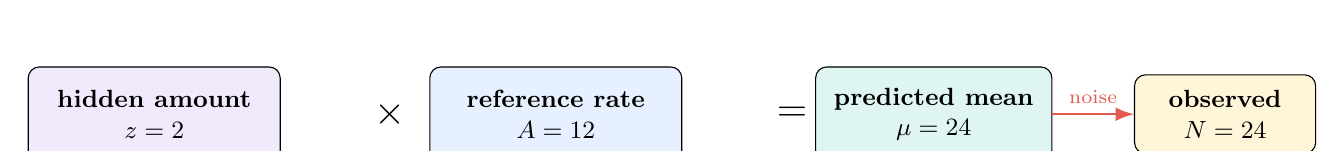
\begin{tikzpicture}[>=Latex,every node/.style={align=center,font=\small}]
  \node[draw,rounded corners,fill=unknownpale,minimum width=3.2cm,minimum height=1.2cm] (z)
    {\textbf{hidden amount}\\\(z=2\)};
  \node[font=\Large] at (3.0,0) {\(\times\)};
  \node[draw,rounded corners,fill=fixedpale,minimum width=3.2cm,minimum height=1.2cm] (a) at (5.1,0)
    {\textbf{reference rate}\\\(A=12\)};
  \node[font=\Large] at (8.1,0) {\(=\)};
  \node[draw,rounded corners,fill=calcpale,minimum width=3.0cm,minimum height=1.2cm] (mu) at (9.9,0)
    {\textbf{predicted mean}\\\(\mu=24\)};
  \node[draw,rounded corners,fill=observedpale,minimum width=2.3cm,minimum height=1.0cm] (n) at (13.6,0)
    {\textbf{observed}\\\(N=24\)};
  \draw[->,thick,coral] (mu.east) -- node[above,font=\scriptsize]{noise} (n.west);
\end{tikzpicture}
\caption{A proposed amount and a known rate produce a predicted mean; the experiment produces an observed count.}
\end{figure}

\begin{checkpoint}
If \(A=5\) cut sites per unit and \(N\) is near 20, what effective abundance is
a sensible first guess?

\textbf{Answer:} \(z\approx20/5=4\).
\end{checkpoint}

\subsection*{Symbol ledger after Level 1}

\begin{center}
\begin{tabular}{C{0.12\linewidth}L{0.38\linewidth}L{0.28\linewidth}}
\toprule
Symbol & Meaning & Role \\
\midrule
\(A\) & reference rate & fixed \\
\(z\) & effective abundance & unknown \\
\(\mu\) & predicted mean count & calculated \\
\(N\) & observed total count & data \\
\bottomrule
\end{tabular}
\end{center}

\section{Level 2: two cell types, still one peak}

Now allow T cells and B cells. We use the letters T and B as readable labels;
the generic cell-type index will come much later.

\[
A_T=12,\qquad A_B=12.
\]

Try this hidden recipe:
\[
z_T=1.5,\qquad z_B=0.5.
\]

The predicted total becomes:
\[
\boxed{\mu=z_TA_T+z_BA_B.}
\]
With the running numbers:
\[
\mu=1.5(12)+0.5(12)=18+6=24.
\]

\begin{translation}
Add the expected T-cell contribution and the expected B-cell contribution to get
the expected peak total.
\end{translation}

\subsection{Why the total alone can be ambiguous}

Because the two reference rates are equal, several recipes predict the same total:

\begin{center}
\begin{tabular}{C{0.22\linewidth}C{0.22\linewidth}C{0.30\linewidth}}
\toprule
\(z_T\) & \(z_B\) & predicted total \(\mu\) \\
\midrule
1.5 & 0.5 & \(1.5(12)+0.5(12)=24\) \\
1.0 & 1.0 & \(1.0(12)+1.0(12)=24\) \\
0.5 & 1.5 & \(0.5(12)+1.5(12)=24\) \\
\bottomrule
\end{tabular}
\end{center}

The peak total reveals that the combined effective amount is about two, but not
which recipe produced it. This is the basic deconvolution problem.

\begin{newvar}{\(\outputq{\pi_T}\) and \(\outputq{\pi_B}\)}
\textbf{Name:} normalized cell-type proportions.\\
\textbf{Job:} convert effective abundances into the reported mixture.\\
\textbf{Range:} between 0 and 1; together they sum to 1.
\end{newvar}

\[
\pi_T=\frac{z_T}{z_T+z_B}
=\frac{1.5}{2}=0.75,
\qquad
\pi_B=\frac{0.5}{2}=0.25.
\]

\begin{watchout}
\(z_T=1.5\) is not “one and a half nuclei.” It is a positive, depth-scaled
reference-cell-equivalent amount. The normalized proportions \(\pi_T,\pi_B\)
are the standardized biological output.
\end{watchout}

\begin{checkpoint}
Why can \(N=24\) not distinguish the three recipes in the table?

\textbf{Answer:} \(A_T=A_B\), so moving one unit from T to B leaves the predicted
total unchanged.
\end{checkpoint}

\section{Level 3: divide the same 24 cuts into length bins}

The peak total hides how its cut sites were distributed by parent-fragment
length. ShapeMix keeps three bins:

\begin{newvar}{\(\calcq{L}\)}
\textbf{Name:} parent-fragment length.\\
\textbf{Job:} determines which length bin both endpoint cut sites inherit.\\
\textbf{Units:} base pairs (bp); later we calculate it as fragment end minus start.
\end{newvar}

\begin{center}
\begin{tabular}{L{0.28\linewidth}L{0.42\linewidth}}
\toprule
Friendly name & Frozen length interval \\
\midrule
short & \(0\le L<100\) bp \\
mono (middle in figures) & \(100\le L<250\) bp \\
long & \(L\ge250\) bp \\
\bottomrule
\end{tabular}
\end{center}

\subsection{First name the observed split}

\begin{newvar}{\(\obsq{\boldsymbol{Y}}\)}
\textbf{Name:} observed bin-count vector.\\
\textbf{Job:} records the short, mono, and long cut-site counts in that order.\\
\textbf{Running value:} \(\boldsymbol{Y}=(10,8,6)\).
\end{newvar}

The bold type means “a list of numbers.” Conservation gives:
\[
N=10+8+6=24.
\]

Under the simplifying picture in which both ends of every fragment land in this
peak, \((10,8,6)\) corresponds to 5 short, 4 mono, and 3 long fragments.

\subsection{Then name the fixed reference shapes}

\begin{newvar}{\(\fixedq{\boldsymbol{\omega}_T}\) and \(\fixedq{\boldsymbol{\omega}_B}\)}
\textbf{Name:} conditional reference length fingerprints.\\
\textbf{Job:} for one cell type and one peak, give the expected fractions in the
short, mono, and long bins.\\
\textbf{Rule:} each vector is fixed from training-reference cells and sums to 1.
\end{newvar}

Use:
\[
\boldsymbol{\omega}_T=
\left(\frac12,\frac13,\frac16\right),
\qquad
\boldsymbol{\omega}_B=
\left(\frac16,\frac13,\frac12\right).
\]

T-cell cuts are more often short-parent; B-cell cuts are more often long-parent.

\subsection{Build the predicted bin counts}

The T contribution is:
\[
z_TA_T\boldsymbol{\omega}_T
=1.5(12)
\left(\frac12,\frac13,\frac16\right)
=(9,6,3).
\]
The B contribution is:
\[
z_BA_B\boldsymbol{\omega}_B
=0.5(12)
\left(\frac16,\frac13,\frac12\right)
=(1,2,3).
\]

\begin{newvar}{\(\calcq{\boldsymbol{v}}\)}
\textbf{Name:} predicted bin-count vector.\\
\textbf{Job:} add all cell-type contributions for each length bin.\\
\textbf{Units:} expected cut sites.\\
\textbf{Running value:} \(\boldsymbol{v}=(10,8,6)\).
\end{newvar}

\[
\boldsymbol{v}=(9,6,3)+(1,2,3)=(10,8,6).
\]

\begin{figure}[H]
\centering
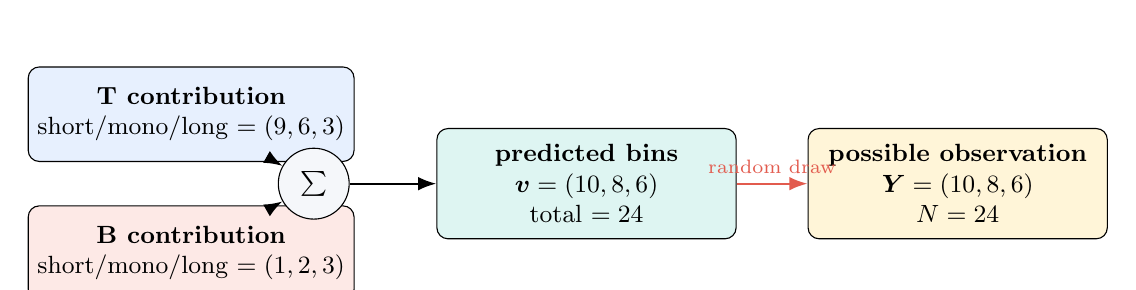
\begin{tikzpicture}[>=Latex,every node/.style={align=center,font=\small}]
  \node[draw,rounded corners,fill=fixedpale,minimum width=3.5cm,minimum height=1.2cm] (t)
    {\textbf{T contribution}\\short/mono/long \(=(9,6,3)\)};
  \node[draw,rounded corners,fill=coralpale,minimum width=3.5cm,minimum height=1.2cm,below=0.55cm of t] (b)
    {\textbf{B contribution}\\short/mono/long \(=(1,2,3)\)};
  \node[draw,circle,fill=lightgray,minimum size=0.9cm,right=1.1cm of $(t)!0.5!(b)$] (sum) {\(\sum\)};
  \node[draw,rounded corners,fill=calcpale,minimum width=3.8cm,minimum height=1.4cm,right=1.1cm of sum] (v)
    {\textbf{predicted bins}\\\(\boldsymbol v=(10,8,6)\)\\total \(=24\)};
  \node[draw,rounded corners,fill=observedpale,minimum width=3.8cm,minimum height=1.4cm,right=0.9cm of v] (y)
    {\textbf{possible observation}\\\(\boldsymbol Y=(10,8,6)\)\\\(N=24\)};
  \draw[->,thick] (t) -- (sum);
  \draw[->,thick] (b) -- (sum);
  \draw[->,thick] (sum) -- (v);
  \draw[->,thick,coral] (v) -- node[above,font=\scriptsize]{random draw} (y);
\end{tikzpicture}
\caption{The predicted bin counts retain information that disappears when they are summed to 24.}
\end{figure}

\begin{newvar}{\(\calcq{\boldsymbol{\rho}}\), pronounced “row”}
\textbf{Name:} predicted bin-probability vector.\\
\textbf{Job:} divide predicted bin counts by their total.\\
\textbf{Rule:} the entries are nonnegative and sum to 1.\\
\textbf{Running value:}
\(\boldsymbol{\rho}=(10,8,6)/24=(5/12,1/3,1/4)\).
\end{newvar}

\[
\boxed{\boldsymbol{\rho}=\frac{\boldsymbol v}{\mu}.}
\]

\subsection{The multinomial asks “how was the total split?”}

After the total \(N=24\) is fixed, the conditional multinomial models how those
same 24 cut sites are allocated:
\[
\boxed{
\boldsymbol{Y}\mid N
\sim
\Mult(N,\boldsymbol{\rho}).
}
\]

The vertical bar means “given.” The tilde means “is modeled as a random draw
from.” This is not 24 new observations: it is a second question about the same
24 cut sites.

\begin{bigidea}
The total asks “how many?” The conditional shape term asks “how split?” When
\(A_T=A_B\), the total cannot distinguish T from B, but the short/mono/long split
can.
\end{bigidea}

\begin{checkpoint}
What extra information does \(\boldsymbol Y\mid N\) contain beyond \(N\)?

\textbf{Answer:} it records how the fixed total was divided among the three
parent-length bins.
\end{checkpoint}

\section{Level 4: observed counts are noisy}

So far the observed values happened to equal the predictions. Real sequencing
counts fluctuate. The model therefore distinguishes:

\[
\underbrace{\mu}_{\text{predicted long-run center}}
\qquad\text{from}\qquad
\underbrace{N}_{\text{one observed total}}.
\]

\begin{newvar}{\(\calcq{e}\)}
\textbf{Name:} total effective abundance.\\
\textbf{Job:} add the effective amounts in the spot.\\
\textbf{Running value:} \(e=z_T+z_B=1.5+0.5=2\).
\end{newvar}

\begin{newvar}{\(\fixedq{\phi_{\mathrm{ref}}}\), pronounced “fye ref”}
\textbf{Name:} reference inverse-dispersion.\\
\textbf{Job:} a fixed training-reference estimate controlling extra variability
in peak totals.\\
\textbf{Direction:} larger inverse-dispersion means less extra variability.\\
\textbf{Example value for this hand calculation:}
use \(\phi_{\mathrm{ref}}=6\). This number is not hard-coded in ShapeMix.
\end{newvar}

\begin{bigidea}
\textbf{What “fixed” means here.} ShapeMix first estimates
\(\phi_{\mathrm{ref}}\) from the training-reference cells. Once that training
step is complete, it holds the estimate fixed while inferring \(z\) for the
mixed spots. A different dataset or training split can produce a different
value. Version 1 freezes the \emph{estimation procedure}, not the numerical value
6; the value 6 is used here only because it makes the arithmetic easy to follow.
\end{bigidea}

Using the tutorial's example value, this spot's inverse-dispersion is
\[
e\phi_{\mathrm{ref}}=2(6)=12.
\]

The peak total is modeled by a negative binomial:
\[
\boxed{
N\sim\NB\!\left(
\text{mean}=\mu,\;
\text{inverse-dispersion}=e\phi_{\mathrm{ref}}
\right).
}
\]

Its variance is:
\[
\Var(N)=\mu+\frac{\mu^2}{e\phi_{\mathrm{ref}}}.
\]
With the running numbers:
\[
\Var(N)=24+\frac{24^2}{12}=24+48=72.
\]

\begin{translation}
Repeated versions of the same experiment would be centered around 24, but they
would not all equal 24. The negative binomial allows more spread than a Poisson
count with the same mean.
\end{translation}

\begin{watchout}
Some writing loosely calls the spot-level quantity
\(e\phi_{\mathrm{ref}}\) “dispersion.” In ShapeMix it behaves as an
\emph{inverse-dispersion}: increasing \(e\phi_{\mathrm{ref}}\) reduces the extra
variance term \(\mu^2/(e\phi_{\mathrm{ref}})\).
\end{watchout}

\begin{center}
\begin{tabularx}{0.91\linewidth}{L{0.25\linewidth}L{0.27\linewidth}X}
\toprule
Distribution & Question & ShapeMix role \\
\midrule
Negative binomial & How many cut sites? & noisy peak total \(N\) \\
Conditional multinomial & How were they split? & bin vector \(\boldsymbol Y\) given \(N\) \\
Gamma & Which positive amounts were plausible beforehand? & prior on \(z\), introduced next \\
\bottomrule
\end{tabularx}
\end{center}

\begin{checkpoint}
If \(\mu=24\), must \(N\) equal 24?

\textbf{Answer:} no. \(\mu\) is the model's center; \(N\) is one noisy observation.
\end{checkpoint}

\section{Level 5: prior, likelihood, posterior, and MAP}

\subsection{The fixed Gamma prior}

Before examining the current spot, ShapeMix assigns the same positive prior to
every cell type's effective abundance:
\[
\boxed{z_T\sim\Gam(\text{shape}=2,\text{rate}=1),\qquad
z_B\sim\Gam(\text{shape}=2,\text{rate}=1).}
\]

This is the frozen version-1 prior. It has mean 2, variance 2, and mode 1.

\begin{figure}[H]
\centering
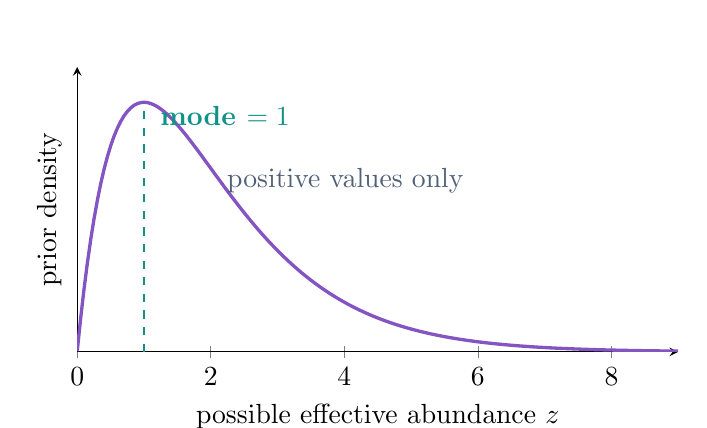
\begin{tikzpicture}
\begin{axis}[
  width=0.76\linewidth,
  height=5.2cm,
  xmin=0,xmax=9,
  ymin=0,ymax=0.42,
  xlabel={possible effective abundance \(z\)},
  ylabel={prior density},
  ytick=\empty,
  axis lines=left,
  samples=180
]
  \addplot[domain=0.001:9,very thick,unknownpurple] {x*exp(-x)};
  \addplot[dashed,calcteal,thick] coordinates {(1,0) (1,0.3679)};
  \node[anchor=south west,text=calcteal,font=\bfseries] at (axis cs:1.1,0.32) {mode \(=1\)};
  \node[anchor=south west,text=slate] at (axis cs:2.1,0.22) {positive values only};
\end{axis}
\end{tikzpicture}
\caption{The \(\Gam(2,1)\) prior is a probability density over positive effective abundance.}
\end{figure}

Because T and B receive the same prior, no named type is favored. The prior does,
however, prefer positive, moderate amounts over values extremely close to zero or
extremely large values.

\begin{watchout}
A prior is a modeling assumption, not a biological fact. Different plausible
priors can yield different posteriors when the data are weak. The protocol freezes
the prior before final evaluation and uses the same prior in both model arms;
scientific sensitivity checks should disclose whether conclusions change under
other predeclared priors.
\end{watchout}

\subsection{How Bayes combines the pieces}

\begin{center}
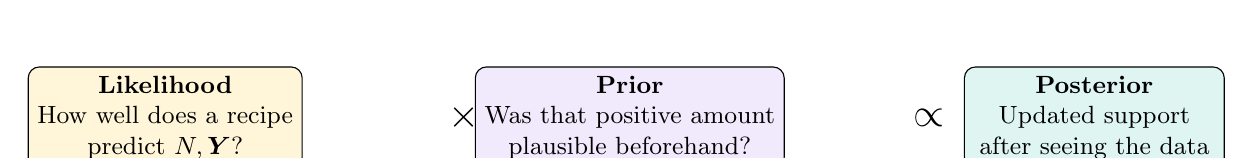
\begin{tikzpicture}[>=Latex,every node/.style={align=center,font=\small}]
  \node[draw,rounded corners,fill=observedpale,minimum width=3.3cm,minimum height=1.2cm] (like)
    {\textbf{Likelihood}\\How well does a recipe\\predict \(N,\boldsymbol Y\)?};
  \node[font=\Large] at (3.8,0) {\(\times\)};
  \node[draw,rounded corners,fill=unknownpale,minimum width=3.3cm,minimum height=1.2cm] (prior) at (5.9,0)
    {\textbf{Prior}\\Was that positive amount\\plausible beforehand?};
  \node[font=\Large] at (9.7,0) {\(\propto\)};
  \node[draw,rounded corners,fill=calcpale,minimum width=3.3cm,minimum height=1.2cm] (post) at (11.8,0)
    {\textbf{Posterior}\\Updated support\\after seeing the data};
\end{tikzpicture}
\end{center}

In symbols:
\[
\underbrace{p(z_T,z_B\mid N,\boldsymbol Y)}_{\text{posterior}}
\propto
\underbrace{p(N,\boldsymbol Y\mid z_T,z_B)}_{\text{likelihood}}
\underbrace{p(z_T)p(z_B)}_{\text{Gamma priors}}.
\]

Here \(p(\cdot)\) means a probability or probability density, the vertical bar
means “given,” and \(\propto\) means “proportional to.”

\begin{newvar}{\(\unknownq{\widehat{\boldsymbol z}_{\mathrm{MAP}}}\)}
\textbf{Name:} maximum-a-posteriori estimate.\\
\textbf{Job:} the single abundance vector at the highest point of the posterior.\\
\textbf{Hat:} a hat means “estimated.”\\
\textbf{MAP:} maximum a posteriori, or “highest posterior.”
\end{newvar}

\[
\widehat{\boldsymbol z}_{\mathrm{MAP}}
=
\arg\max_{\boldsymbol z>0}
\left[
\log p(N,\boldsymbol Y\mid\boldsymbol z)
+\log p(\boldsymbol z)
\right].
\]

The software normalizes this best point to report:
\[
\widehat\pi_T=
\frac{\widehat z_T}{\widehat z_T+\widehat z_B},
\qquad
\widehat\pi_B=
\frac{\widehat z_B}{\widehat z_T+\widehat z_B}.
\]

\begin{watchout}
MAP reports the location of the posterior's highest point, not its width.
Consequently, the MVP does not provide a confidence level or credible interval
for each reported proportion. Optimization diagnostics are not uncertainty
intervals.
\end{watchout}

\begin{checkpoint}
Does a MAP estimate of \(75\%\) T mean “75\% confidence that the spot is T”?

\textbf{Answer:} no. It is a point estimate of the spot's T-like mixture
proportion.
\end{checkpoint}

\section{Level 6: add peaks, spots, bins, and cell types}

The small example used readable labels instead of general indices. We now add one
index at a time because real data contain many peaks and spots.

\subsection{First add multiple peaks}

\begin{newvar}{\(\fixedq{p}\)}
\textbf{Name:} peak index.\\
\textbf{Job:} labels a selected genomic peak: \(p=1,2,\ldots,P\).\\
\textbf{Capital \(P\):} the number of selected peaks.
\end{newvar}

Adding \(p\) turns \(A_T\) into \(A_{T,p}\) and \(\mu\) into \(\mu_p\):
\[
\mu_p=z_TA_{T,p}+z_BA_{B,p}.
\]

\begin{center}
\begin{tabular}{C{0.14\linewidth}C{0.20\linewidth}C{0.20\linewidth}L{0.30\linewidth}}
\toprule
Peak & \(A_{T,p}\) & \(A_{B,p}\) & Teaching purpose \\
\midrule
1 & 12 & 12 & total is ambiguous; shape can help \\
2 & 8 & 16 & total itself helps distinguish types \\
\bottomrule
\end{tabular}
\end{center}

For \(z_T=1.5,z_B=0.5\):
\[
\mu_1=24,\qquad
\mu_2=1.5(8)+0.5(16)=20.
\]

\subsection{Then add multiple spots}

\begin{newvar}{\(\unknownq{s}\)}
\textbf{Name:} spot index.\\
\textbf{Job:} labels a spatial spot: \(s=1,2,\ldots,S\).\\
\textbf{Capital \(S\):} the number of spots.
\end{newvar}

The mixture changes by spot, so \(z_T\) becomes \(z_{s,T}\). Fixed reference
fingerprints do not change by spot.

\begin{center}
\begin{tabular}{L{0.22\linewidth}C{0.20\linewidth}C{0.20\linewidth}C{0.25\linewidth}}
\toprule
Spot & \(z_{s,T}\) & \(z_{s,B}\) & peak-1 predicted bins \\
\midrule
spot 1 & 1.5 & 0.5 & \((10,8,6)\) \\
spot 2 & 0.5 & 1.5 & \((6,8,10)\) \\
\bottomrule
\end{tabular}
\end{center}

\subsubsection*{Are the spot abundances estimated independently?}

Yes---in ShapeMix version 1, each spot receives its own abundance vector and is
scored using that spot's own observed counts.  Spot 1's \(N,Y\) help estimate
\((z_{1,T},z_{1,B})\); spot 2's counts help estimate
\((z_{2,T},z_{2,B})\).  There is no neighbor-to-neighbor abundance term.

\begin{center}
\begin{tabular}{L{0.42\linewidth}L{0.42\linewidth}}
\toprule
Shared across all spots & Different for each spot \\
\midrule
reference peak rates \(A\) & observed counts \(N,Y\) \\
reference length shapes \(\omega\) & inferred abundances \(z\) \\
reference inverse-dispersion \(\phi_{\mathrm{ref}}\) & total effective abundance \(e\) \\
Gamma-prior parameters & predictions \(\mu,\rho\) and output \(\pi\) \\
selected peaks and cell-type definitions & one separate reported mixture row \\
\bottomrule
\end{tabular}
\end{center}

\begin{watchout}
Software may process many spots together in one batch for speed.  Batching is a
computational detail; it does not make one spot's abundance affect another's.
Spatial smoothing and hierarchical coupling are not part of version 1.
\end{watchout}

\subsection{Finally replace names with general indices}

\begin{newvar}{\(\fixedq{b}\) and \(\unknownq{c}\)}
\(b=1,\ldots,B\) labels a parent-length bin; version 1 has \(B=3\).\\
\(c=1,\ldots,C\) labels a declared cell type; \(C\) is the number of types.\\
The earlier T and B labels are simply two possible values of \(c\).
\end{newvar}

\begin{center}
\begin{tabular}{C{0.11\linewidth}L{0.66\linewidth}}
\toprule
Index & Meaning \\
\midrule
\(s\) & which spatial spot? \\
\(p\) & which selected genomic peak? \\
\(b\) & which parent-fragment length bin? \\
\(c\) & which reference cell type? \\
\bottomrule
\end{tabular}
\end{center}

Examples:

\begin{itemize}[leftmargin=2em]
  \item \(Y_{3,12,2}\): observed cut-site count in spot 3, peak 12, bin 2.
  \item \(A_{T,12}\): fixed T-reference total rate at peak 12.
  \item \(\omega_{B,12,3}\): fixed B-reference long-bin fraction at peak 12.
  \item \(z_{3,T}\): inferred T-like effective abundance in spot 3.
\end{itemize}

\begin{watchout}
The italic subscript \(p\) labels a peak. The notation \(p(\cdot)\) used in the
Bayes section denotes a probability density. Context distinguishes them.
\end{watchout}

\subsection{Array shapes before equations}

\begin{center}
\begin{tabular}{L{0.25\linewidth}C{0.27\linewidth}L{0.31\linewidth}}
\toprule
Quantity & Dimensions & Role \\
\midrule
\(z\) & \(S\times C\) & inferred spot-by-type amounts \\
\(A\) & \(C\times P\) & fixed type-by-peak rates \\
\(\omega\) & \(C\times P\times B\) & fixed type-by-peak-by-bin fractions \\
\(N,\mu\) & \(S\times P\) & observed and predicted peak totals \\
\(Y,v,\rho\) & \(S\times P\times B\) & observed counts, predicted counts, predicted fractions \\
\bottomrule
\end{tabular}
\end{center}

\section{The complete model, one line at a time}

\subsection{Line 1: total effective abundance}

\[
\boxed{e_s=\sum_cz_{s,c}.}
\]

\begin{translation}
For one spot, add the effective amounts across all declared cell types.
\end{translation}

\subsection{Line 2: predicted count in one length bin}

\[
\boxed{
v_{s,p,b}
=
\sum_cz_{s,c}A_{c,p}\omega_{c,p,b}.
}
\]

\begin{translation}
For one spot, peak, and length bin, calculate every cell type's contribution and
add them.
\[
\underbrace{z}_{\text{effective units}}
\times
\underbrace{A}_{\text{cuts/unit}}
\times
\underbrace{\omega}_{\text{fraction}}
=
\underbrace{v}_{\text{expected cuts}}.
\]
\end{translation}

\subsection{Line 3: predicted total and bin fractions}

\[
\boxed{
\mu_{s,p}=\sum_bv_{s,p,b},
\qquad
\rho_{s,p,b}=\frac{v_{s,p,b}}{\mu_{s,p}}.
}
\]

\begin{translation}
Add the predicted bins to get the predicted peak total. Divide each predicted bin
by that total to obtain fractions that sum to one.
\end{translation}

\subsection{Line 4: noisy observed peak total}

\begin{newvar}{\(\fixedq{\epsilon}\), pronounced “epsilon”}
\textbf{Name:} numerical safety floor.\\
\textbf{Job:} a small fixed positive number that prevents invalid zero
inverse-dispersion during computation. It is not inferred from the spot.
\end{newvar}

\[
\boxed{
N_{s,p}
\sim
\NB\!\left(
\text{mean}=\mu_{s,p},\;
\text{inverse-dispersion}
=\max(e_s,\epsilon)\phi_{\mathrm{ref}}
\right).
}
\]

\begin{translation}
The observed peak total is a noisy count around the predicted mean. Larger spots
receive the abundance-scaled inverse-dispersion required by the version-1 model.
\end{translation}

\subsection{Line 5: conditional length-bin split}

\[
\boxed{
\boldsymbol Y_{s,p,\boldsymbol\cdot}\mid N_{s,p}
\sim
\Mult\!\left(
N_{s,p},
\boldsymbol\rho_{s,p,\boldsymbol\cdot}
\right).
}
\]

The bold dot means “take the complete vector over all bins while holding \(s\)
and \(p\) fixed.”

\begin{translation}
Given the observed peak total, allocate those same cut sites among the three
length bins according to the predicted fractions.
\end{translation}

\subsection{Line 6: prior and reported proportions}

\[
\boxed{
z_{s,c}\sim\Gam(2,1),
\qquad
\pi_{s,c}=\frac{z_{s,c}}{e_s}.
}
\]

\begin{translation}
Give every cell type the same fixed positive prior, infer the MAP abundances, and
normalize them so each spot's reported proportions sum to one.
\end{translation}

\subsection{Why the MAP calculation separates by spot}

After all indices have been introduced, the MAP score can be written as a sum of
one score for each spot:
\[
\begin{aligned}
\text{total MAP score}
&=\sum_s \text{spot score}_s,\\[2pt]
\text{spot score}_s
&=\sum_p\left[
  \log p(N_{s,p}\mid z_s)
  +\log p(\boldsymbol Y_{s,p,\cdot}\mid N_{s,p},z_s)
  \right]
  +\sum_c\log p(z_{s,c}).
\end{aligned}
\]

The first sum measures how well \(z_s\) explains every peak in spot \(s\); the
last sum supplies that spot's Gamma-prior score.  The fixed
\(A,\omega,\phi_{\mathrm{ref}}\) are shared by all spots and are left implicit in
the probability notation.

No spot score contains another spot's abundance.  Consequently, maximizing the
total score is mathematically equivalent to maximizing each spot's score
separately, conditional on the shared reference quantities.  Each reported row
is then normalized within its own spot:
\[
\widehat\pi_{s,c}
=
\frac{\widehat z_{s,c}}{\sum_{c'}\widehat z_{s,c'}}.
\]
Here \(c'\) is only a dummy summation label: the denominator adds the estimated
abundances over every declared cell type in the same spot.

\subsection{One generative diagram}

\begin{figure}[H]
\centering
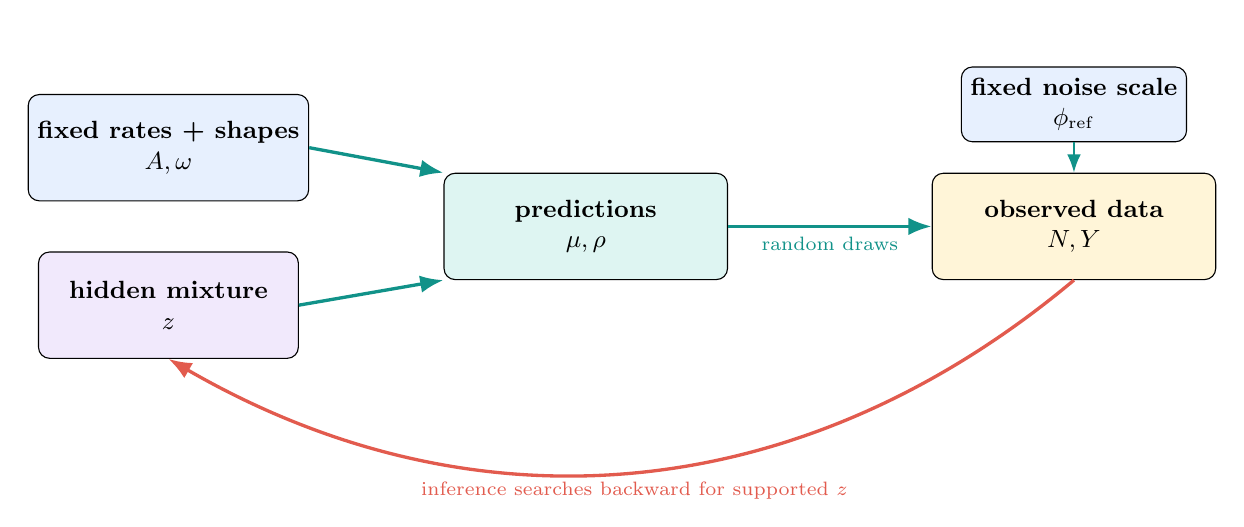
\begin{tikzpicture}[>=Latex,every node/.style={align=center,font=\small}]
  \node[draw,rounded corners,fill=fixedpale,minimum width=3.3cm,minimum height=1.35cm] (ref) at (0,1.0)
    {\textbf{fixed rates + shapes}\\\(A,\omega\)};
  \node[draw,rounded corners,fill=unknownpale,minimum width=3.3cm,minimum height=1.35cm] (z) at (0,-1.0)
    {\textbf{hidden mixture}\\\(z\)};
  \node[draw,rounded corners,fill=calcpale,minimum width=3.6cm,minimum height=1.35cm] (pred) at (5.3,0)
    {\textbf{predictions}\\\(\mu,\rho\)};
  \node[draw,rounded corners,fill=fixedpale,minimum width=2.6cm,minimum height=0.95cm] (noise) at (11.5,1.55)
    {\textbf{fixed noise scale}\\\(\phi_{\mathrm{ref}}\)};
  \node[draw,rounded corners,fill=observedpale,minimum width=3.6cm,minimum height=1.35cm] (data) at (11.5,0)
    {\textbf{observed data}\\\(N,Y\)};
  \draw[->,very thick,calcteal] (ref.east) -- (pred.north west);
  \draw[->,very thick,calcteal] (z.east) -- (pred.south west);
  \draw[->,very thick,calcteal] (pred) --
    node[below,font=\scriptsize]{random draws} (data);
  \draw[->,thick,calcteal] (noise.south) -- (data.north);
  \draw[->,very thick,coral,bend left=35] (data.south) to
    node[below,font=\scriptsize]{inference searches backward for supported \(z\)}
    (z.south);
\end{tikzpicture}
\caption{The model runs forward from a candidate mixture to possible data; MAP inference uses observed data to search backward.}
\end{figure}

\subsubsection*{What does “generative” mean?}

A \emph{generative model} is a mathematical recipe for how the model imagines
that observable data could be produced.  The forward, teal arrows in Figure~5
tell this story:

\begin{enumerate}[leftmargin=2em]
  \item Start with one possible hidden mixture \(z\).
  \item Combine \(z\) with the fixed reference rates and shapes \(A,\omega\) to
  calculate the predicted total \(\mu\) and predicted bin fractions \(\rho\).
  \item Allow random experimental variation, controlled partly by
  \(\phi_{\mathrm{ref}}\), to produce possible observed counts \(N,Y\).
\end{enumerate}

The boxes therefore have these jobs:

\begin{center}
\begin{tabular}{C{0.16\linewidth}L{0.66\linewidth}}
\toprule
Box & Meaning \\
\midrule
\(z\) & hidden effective cell-type amounts \\
\(A,\omega\) & fixed reference information that turns a mixture into count and shape predictions \\
\(\mu,\rho\) & predicted peak total and predicted short/mono/long fractions \\
\(\phi_{\mathrm{ref}}\) & fixed reference noise scale used in the negative-binomial draw \\
\(N,Y\) & total and length-bin counts actually observed \\
\bottomrule
\end{tabular}
\end{center}

For the running example, one candidate mixture is
\[
z_T=1.5,\qquad z_B=0.5.
\]
Running this candidate \emph{forward} through the model gives
\[
\mu=24,
\qquad
\rho=\left(\frac{10}{24},\frac{8}{24},\frac{6}{24}\right).
\]
A possible observation is then
\[
N=24,
\qquad
Y=(10,8,6).
\]

\subsubsection*{What does “inference searches backward” mean?}

In a real experiment, the direction of the problem is reversed: we already know
the observed \(N,Y\), but we do not know the hidden \(z\).  ShapeMix therefore
tries candidate values of \(z\) and asks:

\begin{quote}
\emph{If this were the mixture, how well would it explain the counts that we
observed?}
\end{quote}

For \(N=24\) and \(Y=(10,8,6)\), three candidates with the same total effective
amount predict different shapes:

\begin{center}
\begin{tabular}{C{0.18\linewidth}C{0.22\linewidth}C{0.26\linewidth}L{0.16\linewidth}}
\toprule
T proportion & \((z_T,z_B)\) & predicted short/mono/long & match \\
\midrule
25\% & \((0.5,1.5)\) & \((6,8,10)\) & weak \\
50\% & \((1.0,1.0)\) & \((8,8,8)\) & intermediate \\
75\% & \((1.5,0.5)\) & \((10,8,6)\) & strongest \\
\bottomrule
\end{tabular}
\end{center}

The software repeats the following search:

\begin{enumerate}[leftmargin=2em]
  \item propose a possible \(z\);
  \item run that \(z\) forward to calculate \(\mu,\rho\);
  \item score how well those predictions explain the observed \(N,Y\);
  \item include how plausible the candidate is under the Gamma prior; and
  \item move toward a higher posterior score until it finds the MAP estimate.
\end{enumerate}

\begin{watchout}
The red arrow is not a claim that biology or time literally runs backward.  It
shows the direction of the computer's reasoning: from known observations toward
an unknown explanation.  A “supported \(z\)” is a candidate that explains the
data well \emph{and} is reasonably compatible with the prior.  The MAP result is
the highest-scoring point, not a confidence interval.
\end{watchout}

\subsection{How one candidate \(z\) receives a likelihood score}

For a proposed \(z\), ShapeMix calculates the probability of the observed data
in two parts:
\[
\boxed{
\underbrace{p(N,\boldsymbol Y\mid z)}_{\text{data likelihood}}
=
\underbrace{p(N\mid z)}_{\text{total-count score}}
\times
\underbrace{p(\boldsymbol Y\mid N,z)}_{\text{bin-split score}}.
}
\]

These are probability \emph{masses}: they score the exact integer counts that
were observed.  The two factors answer different questions.

\subsubsection*{Part 1: score the observed total with a negative binomial}

The candidate \(z\) determines \(e\) and the predicted mean \(\mu\). ShapeMix
evaluates the negative-binomial probability at the observed total \(N\):
\[
p(N\mid z)
=
\NB\!\left(
N;\ \text{mean}=\mu,\
\text{inverse-dispersion}=\max(e,\epsilon)\phi_{\mathrm{ref}}
\right).
\]

For the running candidate, \(\mu=24\), \(e=2\), and the tutorial uses
\(\phi_{\mathrm{ref}}=6\).  The distribution is therefore centered at 24 with
inverse-dispersion 12.  Observing \(N=24\) receives a relatively high total-count
score.  A distant value such as \(N=60\) receives a much lower score, but not
necessarily zero, because the model allows experimental noise.

\subsubsection*{Part 2: score the observed split with a multinomial}

The same candidate predicts the fractions
\[
\boldsymbol\rho
=
(\rho_{\mathrm{short}},\rho_{\mathrm{mono}},\rho_{\mathrm{long}}).
\]
Given that exactly \(N\) cuts were observed, the multinomial asks how plausible
their allocation among the three bins was:
\[
p(\boldsymbol Y\mid N,z)
=
\frac{N!}{Y_{\mathrm{short}}!Y_{\mathrm{mono}}!Y_{\mathrm{long}}!}
\prod_b\rho_b^{Y_b}.
\]

For \(N=24\), \(\boldsymbol Y=(10,8,6)\), and
\(\boldsymbol\rho=(10/24,8/24,6/24)\), this becomes
\[
\begin{aligned}
p((10,8,6)\mid N=24,z)
&=\frac{24!}{10!\,8!\,6!}
\left(\frac{10}{24}\right)^{10}
\left(\frac{8}{24}\right)^8
\left(\frac{6}{24}\right)^6.
\end{aligned}
\]
The factorial factor counts all possible orders in which 10 short, 8 mono, and
6 long cuts could have appeared.  This is like asking for the chance of seeing
particular color totals after 24 random draws from three colored bins.

The candidate predicting \((10,8,6)\) receives a higher shape likelihood than
candidates predicting \((8,8,8)\) or \((6,8,10)\).  Exact equality is not a
requirement: the multinomial assigns probabilities to many possible allocations.

\subsubsection*{Combine peaks, then add the prior}

For many peaks, ShapeMix multiplies the two likelihood factors across peaks.  In
software it adds logarithms, which is numerically safer:
\[
\log p(N,\boldsymbol Y\mid z)
=
\sum_p\left[
\log p(N_p\mid z)
+
\log p(\boldsymbol Y_{p,\cdot}\mid N_p,z)
\right].
\]
The likelihood is the data-fit score. MAP then adds the Gamma-prior score:
\[
\underbrace{\log p(N,\boldsymbol Y\mid z)}_{\text{fit to the observed data}}
+
\underbrace{\log p(z)}_{\text{prior plausibility}}
=
\text{posterior score, up to a constant}.
\]

\begin{watchout}
The likelihood \(p(N,\boldsymbol Y\mid z)\) means “how probable were these data
if this \(z\) were used?” It is not the probability that \(z\) is true.  The
posterior combines that likelihood with the prior.  A candidate that exactly
matches one peak is not automatically the MAP estimate: all peaks, count noise,
and the Gamma prior contribute to the final score.
\end{watchout}

\subsection{Count-only versus ShapeMix}

Both arms use the same observed totals, reference signatures, prior,
initialization, optimizer, seeds, and compute budget.

\begin{center}
\begin{tabular}{L{0.31\linewidth}C{0.20\linewidth}C{0.20\linewidth}}
\toprule
Term & Count-only & ShapeMix \\
\midrule
negative-binomial total likelihood & yes & yes \\
conditional multinomial shape likelihood & no & yes \\
Gamma prior on \(z\) & yes & yes \\
\bottomrule
\end{tabular}
\end{center}

The factorization in the preceding subsection does not double-count
observations. It separates total-count information from allocation information.

\begin{checkpoint}
If every cell type has exactly the same \(\omega_{c,p,\cdot}\), can the shape term
identify the mixture?

\textbf{Answer:} no. Then the predicted bin fractions do not change with \(z\),
so ShapeMix should agree with count-only within numerical tolerance.
\end{checkpoint}

\section{Where the fixed reference quantities come from}

You can understand and use the core model without memorizing this section's
estimation formulas. Its purpose is to show why \(A\), \(\omega\), and
\(\phi_{\mathrm{ref}}\) are fixed before a held-out spot is analyzed.

\subsection{The missing index: an individual reference cell}

\begin{newvar}{\(\fixedq{i}\)}
\textbf{Name:} training-reference cell index.\\
\textbf{Job:} labels one individually measured, cell-type-labeled reference cell.\\
It is different from \(c\): \(i\) identifies one cell; \(c\) identifies its type.
\end{newvar}

\begin{newvar}{\(\obsq{R_{i,p,b}}\) and \(\obsq{T_{i,p}}\)}
\(R_{i,p,b}\) is the training-reference cut-site count for cell \(i\), peak \(p\),
and bin \(b\).\\
\(T_{i,p}=\sum_bR_{i,p,b}\) is that reference cell's total at the peak.
\end{newvar}

If reference cell 17 is labeled T and \(R_{17,42,\mathrm{short}}=3\), that cell
contributed three short-parent cut sites to peak 42.

Let \(\mathcal I_c\) denote the set of training-reference cells labeled as type
\(c\). Conceptually:

\[
A_{c,p}
\approx
\text{average of }T_{i,p}\text{ over }i\in\mathcal I_c,
\]
\[
\omega_{c,p,b}
\approx
\frac{\text{bin-}b\text{ counts pooled over }i\in\mathcal I_c}
{\text{all-bin counts pooled over }i\in\mathcal I_c}.
\]

The actual estimates use frozen smoothing so sparse peaks never receive unstable
zero probabilities. Exact formulas appear in Appendix~\ref{app:reference}.

\subsection{Why dispersion is cross-fitted}

To estimate \(\phi_{\mathrm{ref}}\), ShapeMix splits training-reference cells into
two deterministic folds within each cell type. Each cell is compared with a mean
learned from the opposite fold. This prevents a cell from helping construct the
same mean used to measure its own deviation.

\begin{bigidea}
Reference signatures, smoothing, peak selection, and dispersion use training
reference cells only. Held-out source cells and pseudo-spots cannot influence
them.
\end{bigidea}

\section{What the software reports for each spot}

The current MAP implementation emits:

\begin{center}
\begin{tabularx}{0.94\linewidth}{L{0.25\linewidth}L{0.30\linewidth}X}
\toprule
Output & Contents & Interpretation \\
\midrule
\texttt{abundance.csv} & \(\widehat z_{s,c}\) & effective, depth-scaled MAP abundances; not calibrated nuclei \\
\texttt{proportions.csv} & \(\widehat\pi_{s,c}\) & main composition estimate; each row sums to one \\
\texttt{diagnostics.json} & objectives, restarts, convergence and runtime information & fit diagnostics, not confidence intervals \\
\bottomrule
\end{tabularx}
\end{center}

For example:

\begin{center}
\begin{tabular}{L{0.20\linewidth}C{0.18\linewidth}C{0.18\linewidth}C{0.18\linewidth}}
\toprule
Spot & T & B & Monocyte \\
\midrule
spot 1 & 0.65 & 0.25 & 0.10 \\
spot 2 & 0.15 & 0.70 & 0.15 \\
\bottomrule
\end{tabular}
\end{center}

These rows look like probability vectors mathematically, but scientifically they
are estimated mixture fractions. A value of \(0.65\) does not mean “65\%
confidence.” Spot-level credible intervals would require a new model version that
approximates or samples the posterior rather than reporting only its maximum.

\section{How the observed tensor is constructed}

\subsection{From a fragment row to cut-site counts}

The primary input is a BGZF/tabix-indexed five-column 10x fragments file:
chromosome, start, end, barcode, and \texttt{readSupport}.

\begin{enumerate}[leftmargin=2em]
  \item Treat each row as one deduplicated fragment.
  \item Ignore \texttt{readSupport} in the primary analysis so PCR support is not
  counted again.
  \item Compute parent length \(L=\texttt{end}-\texttt{start}\).
  \item Give both endpoint cut sites the same parent-length bin.
  \item Assign each endpoint independently to the unique selected,
  non-overlapping peak that contains it.
  \item Store one sparse spot-by-peak matrix per length bin.
  \item Require their elementwise sum to equal the ordinary peak-count matrix.
\end{enumerate}

\begin{figure}[H]
\centering
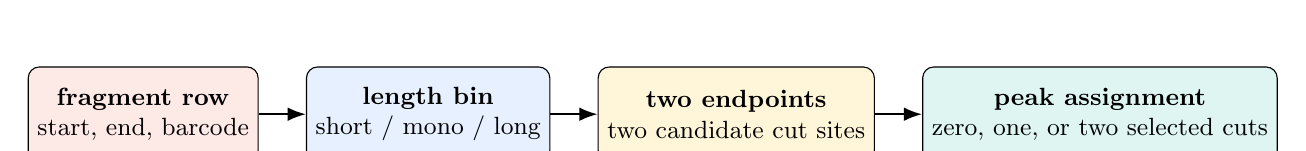
\begin{tikzpicture}[>=Latex,every node/.style={align=center,font=\small}]
  \node[draw,rounded corners,fill=coralpale,minimum width=2.85cm,minimum height=1.2cm] (frag)
    {\textbf{fragment row}\\start, end, barcode};
  \node[draw,rounded corners,fill=fixedpale,minimum width=2.85cm,minimum height=1.2cm,right=0.6cm of frag] (bin)
    {\textbf{length bin}\\short / mono / long};
  \node[draw,rounded corners,fill=observedpale,minimum width=2.85cm,minimum height=1.2cm,right=0.6cm of bin] (cuts)
    {\textbf{two endpoints}\\two candidate cut sites};
  \node[draw,rounded corners,fill=calcpale,minimum width=2.85cm,minimum height=1.2cm,right=0.6cm of cuts] (peak)
    {\textbf{peak assignment}\\zero, one, or two selected cuts};
  \draw[->,thick] (frag) -- (bin);
  \draw[->,thick] (bin) -- (cuts);
  \draw[->,thick] (cuts) -- (peak);
\end{tikzpicture}
\caption{Each fragment is separated before its two endpoints are assigned; overlapping bars are never treated as one long fragment.}
\end{figure}

Version 1 selects 5,000 peaks by a deterministic accessibility-variance rank
computed from reference cells only. Alternative peak counts and length cutoffs
are versioned sensitivity analyses.

\section{A fair experiment: isolate what shape adds}

\subsection{Leakage-free split}

The primary PBMC source contains one donor. Each outer seed makes a deterministic,
cell-type-stratified 70/30 split:

\begin{itemize}[leftmargin=2em]
  \item the 70\% training-reference pool selects peaks and estimates
  \(A,\omega,\phi_{\mathrm{ref}}\);
  \item the held-out 30\% pool supplies cells for pseudo-spots; and
  \item inner mixture seeds are nested inside each outer split.
\end{itemize}

Both arms analyze the exact same pseudo-spots for every paired run. This design
measures conditional resampling variability within one donor; it does not establish
donor-level generalization.

\subsection{Diagnostics and negative controls}

After fitting, check:

\begin{itemize}[leftmargin=2em]
  \item bin layers sum exactly to the ordinary peak totals;
  \item predicted totals \(\mu\) reconstruct \(N\) reasonably;
  \item predicted bin fractions \(\rho\) reconstruct short/mono/long patterns;
  \item objectives, gradients, abundances, and proportions are finite;
  \item restarts converge to compatible solutions;
  \item homogenized \(\omega\) removes ShapeMix's advantage; and
  \item permuted cell-type shape labels do not create a false improvement.
\end{itemize}

\subsection{Primary comparison}

The narrow claim is:

\begin{bigidea}
Does the conditional parent-fragment length composition of the same observed cut
sites improve cell-type proportion estimates beyond their peak totals?
\end{bigidea}

Primary metrics compare \(\widehat\pi\) with known pseudo-spot truth using RMSE and
versioned Jensen--Shannon divergence. Runtime, memory, convergence, per-type
errors, and rare-cell metrics are also reported even if shape does not help.

\section{End-to-end worked example}

We now repeat the entire running example without introducing any new symbols.

\subsection{Step 1: fixed reference information}

\[
A_T=A_B=12,
\]
\[
\boldsymbol\omega_T=
\left(\frac12,\frac13,\frac16\right),
\qquad
\boldsymbol\omega_B=
\left(\frac16,\frac13,\frac12\right).
\]

\subsection{Step 2: one candidate hidden mixture}

\[
z_T=1.5,\qquad z_B=0.5,\qquad e=2.
\]
Therefore:
\[
\pi_T=0.75,\qquad\pi_B=0.25.
\]

\subsection{Step 3: predicted total}

\[
\mu=1.5(12)+0.5(12)=24.
\]

\subsection{Step 4: predicted length split}

\[
\boldsymbol v
=1.5(12)\boldsymbol\omega_T+0.5(12)\boldsymbol\omega_B
=(10,8,6),
\]
\[
\boldsymbol\rho
=\frac{(10,8,6)}{24}
=\left(\frac5{12},\frac13,\frac14\right).
\]

\subsection{Step 5: possible observation}

\[
N=24,\qquad\boldsymbol Y=(10,8,6).
\]
The observation happens to equal the prediction so the arithmetic is transparent;
real observations fluctuate around their predictions.

\subsection{Step 6: why shape identifies the recipe}

Hold \(e=2\) fixed and compare three candidate T proportions:

\begin{center}
\begin{tabular}{C{0.20\linewidth}C{0.23\linewidth}C{0.28\linewidth}}
\toprule
\(\pi_T\) & \((z_T,z_B)\) & predicted short/mono/long \\
\midrule
25\% & \((0.5,1.5)\) & \((6,8,10)\) \\
50\% & \((1.0,1.0)\) & \((8,8,8)\) \\
75\% & \((1.5,0.5)\) & \((10,8,6)\) \\
\bottomrule
\end{tabular}
\end{center}

All three candidates predict the same total, 24. The observed shape
\((10,8,6)\) matches the 75\% T candidate most closely.

\begin{figure}[H]
\centering
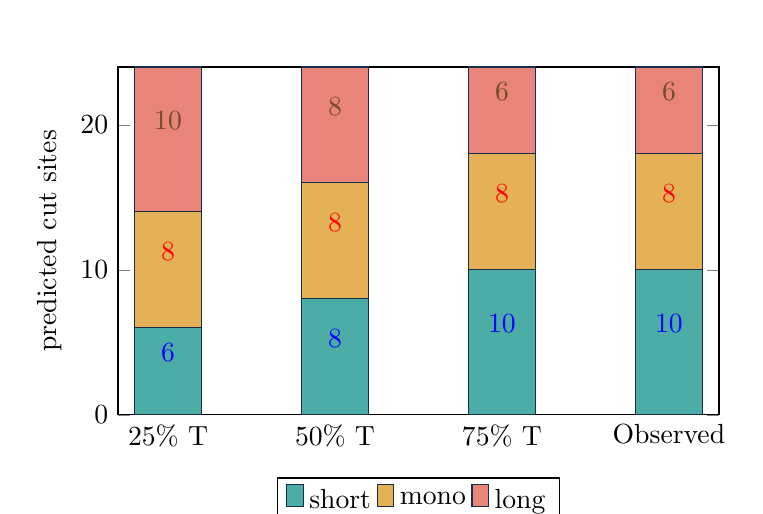
\begin{tikzpicture}
\begin{axis}[
  ybar stacked,
  bar width=24pt,
  width=0.76\linewidth,
  height=6cm,
  ymin=0,ymax=24,
  ylabel={predicted cut sites},
  symbolic x coords={25\% T,50\% T,75\% T,Observed},
  xtick=data,
  legend style={at={(0.5,-0.18)},anchor=north,legend columns=3},
  nodes near coords,
  nodes near coords align={vertical}
]
  \addplot+[fill=calcteal!75,draw=navy] coordinates {(25\% T,6) (50\% T,8) (75\% T,10) (Observed,10)};
  \addplot+[fill=observedgold!75,draw=navy] coordinates {(25\% T,8) (50\% T,8) (75\% T,8) (Observed,8)};
  \addplot+[fill=coral!75,draw=navy] coordinates {(25\% T,10) (50\% T,8) (75\% T,6) (Observed,6)};
  \legend{short,mono,long}
\end{axis}
\end{tikzpicture}
\caption{Peak totals are identical, but the length composition distinguishes the candidate recipes.}
\end{figure}

\begin{watchout}
This exact match is a teaching calculation, not the complete MAP computation.
The implemented result balances negative-binomial total fit, conditional
multinomial shape fit, and the Gamma prior over continuous positive abundances.
\end{watchout}

\section{Symbol glossary in the order learned}

\begin{longtable}{C{0.12\linewidth}L{0.43\linewidth}L{0.30\linewidth}}
\caption{Core symbols, ordered by first conceptual appearance.}\label{tab:glossary}\\
\toprule
Symbol & Meaning & Role \\
\midrule
\endfirsthead
\toprule
Symbol & Meaning & Role \\
\midrule
\endhead
\(A\) & reference peak rate & fixed reference input \\
\(z\) & effective abundance & inferred by MAP \\
\(\mu\) & predicted mean peak total & calculated \\
\(N\) & observed peak total & data \\
\(\pi\) & normalized cell-type proportion & reported output \\
\(\boldsymbol Y\) & observed vector of length-bin counts & data \\
\(\boldsymbol\omega\) & reference conditional length fingerprint & fixed reference input \\
\(\boldsymbol v\) & predicted length-bin counts & calculated \\
\(\boldsymbol\rho\) & predicted length-bin fractions & calculated \\
\(e\) & total effective abundance & calculated \\
\(\phi_{\mathrm{ref}}\) & reference inverse-dispersion & fixed reference input \\
\(p\) & selected-peak index & index \\
\(s\) & spatial-spot index & index \\
\(b\) & parent-length-bin index & index \\
\(c\) & cell-type index & index \\
\(\epsilon\) & small positive numerical guard & fixed setting \\
\(i\) & individual training-reference cell index & index \\
\(R_{i,p,b}\) & training-reference bin count & observed reference data \\
\(T_{i,p}\) & training-reference peak total & observed, calculated from \(R\) \\
\bottomrule
\end{longtable}

\subsection*{Notation operators}

\begin{center}
\begin{tabular}{C{0.18\linewidth}L{0.64\linewidth}}
\toprule
Notation & Read it as \\
\midrule
\(\sum_c\) & add over all cell types \\
\(\sim\) & is modeled as a random draw from \\
\(\mid\) & given \\
\(\propto\) & proportional to \\
\(\widehat z\) & estimated \(z\) \\
\(\arg\max_z f(z)\) & the value of \(z\) where \(f\) is highest \\
\(\boldsymbol Y_{s,p,\boldsymbol\cdot}\) & the complete bin vector for one spot and peak \\
\bottomrule
\end{tabular}
\end{center}

\textbf{About primes on indices:} a primed letter inside a sum is only a dummy
counter. For example, \(\sum_{b'}\) means “add over every bin,” and
\(\sum_{c'}\) means “add over every cell type.” It does not create a new kind of
bin or cell type.

\begin{checkpoint}
You understand the core ShapeMix model if you can explain these six lines in
ordinary language:
\[
\begin{aligned}
v_{s,p,b}&=\sum_cz_{s,c}A_{c,p}\omega_{c,p,b}, &
\mu_{s,p}&=\sum_bv_{s,p,b}, &
\rho_{s,p,b}&=\frac{v_{s,p,b}}{\mu_{s,p}}.
\end{aligned}
\]
\[
\begin{aligned}
N_{s,p}&\sim\NB\!\left(\mu_{s,p},\max(e_s,\epsilon)\phi_{\mathrm{ref}}\right),\\
\boldsymbol Y_{s,p,\cdot}\mid N_{s,p}
&\sim\Mult(N_{s,p},\boldsymbol\rho_{s,p,\cdot}),
& \pi_{s,c}&=\frac{z_{s,c}}{e_s}.
\end{aligned}
\]
\end{checkpoint}

\appendix

\section{Exact fixed-reference estimation}
\label{app:reference}

This appendix matches the executable specification. It is intentionally placed
after the core model because its extra variables describe how fixed inputs are
constructed, not what is inferred for a spot.

For cell type \(c\), let \(\mathcal I_c\) be its training-reference cells and
let \(h_i=1\) be the same-protocol exposure. Define the pooled peak target:
\[
g_p=\frac{\sum_iT_{i,p}}{\sum_ih_i}.
\]
With \(\alpha_A=0.5\):
\[
A_{c,p}
=
\frac{\sum_{i\in\mathcal I_c}T_{i,p}+\alpha_Ag_p}
{\sum_{i\in\mathcal I_c}h_i+\alpha_A}.
\]

Define the dataset-global length distribution:
\[
u_b^{\mathrm{global}}
=
\frac{\sum_{i,p}R_{i,p,b}}
{\sum_{i,p,b'}R_{i,p,b'}}.
\]
With the frozen \(\alpha_\omega=1\), first smooth each pooled peak:
\[
u_{p,b}
=
\frac{\sum_iR_{i,p,b}+\alpha_\omega u_b^{\mathrm{global}}}
{\sum_{i,b'}R_{i,p,b'}+\alpha_\omega},
\]
then smooth each cell-type/peak fingerprint:
\[
\omega_{c,p,b}
=
\frac{\sum_{i\in\mathcal I_c}R_{i,p,b}
+\alpha_\omega u_{p,b}}
{\sum_{i\in\mathcal I_c}T_{i,p}
+\alpha_\omega}.
\]

\begin{translation}
Sparse cell-type/peak observations borrow a small amount of information from the
pooled peak pattern, which itself borrows from the dataset-global pattern. This
keeps every conditional bin probability finite and positive.
\end{translation}

\subsection{Cross-fitted inverse-dispersion}

For each reference cell \(i\), estimate a held-out mean \(m_{i,p}\) from the
opposite within-type fold. Then:
\[
\alpha_{\mathrm{ref}}^{\mathrm{raw}}
=
\frac{\sum_{i,p}\left[(T_{i,p}-m_{i,p})^2-m_{i,p}\right]}
{\sum_{i,p}m_{i,p}^2},
\]
\[
\alpha_{\mathrm{ref}}
=
\max\!\left(\alpha_{\mathrm{ref}}^{\mathrm{raw}},10^{-8}\right),
\qquad
\phi_{\mathrm{ref}}=\frac{1}{\alpha_{\mathrm{ref}}}.
\]

The fold seed, numerator, denominator, and result are recorded. Non-finite values
or a zero denominator are errors.

\section{Optimization, implementation, and fixed contract}

\subsection{MAP fitting}

Only \(z\) is inferred. The implementation uses
\[
z=\operatorname{softplus}(z^{\mathrm{raw}})+\epsilon
\]
to keep abundances positive. It initializes from collapsed-count NNLS with a
uniform fallback, uses deterministic restarts and Adam optimization, processes
spots and peaks in chunks, and fails on non-finite losses, gradients, abundances,
or proportions.

\begin{advanced}{objective comparison}
\[
\mathcal L_{\mathrm{count}}(z)
=
\log p(N\mid z,A,\phi_{\mathrm{ref}})
+\log p(z),
\]
\[
\mathcal L_{\mathrm{shape}}(z)
=
\mathcal L_{\mathrm{count}}(z)
+\log p(Y\mid N,z,A,\omega).
\]
Only the final conditional-shape term differs.
\end{advanced}

\subsection{Sparse implementation invariants}

\begin{itemize}[leftmargin=2em]
  \item Reference and spatial objects have identical ordered selected peaks.
  \item The three ordered CSR layers are short, mono, and long.
  \item Every layer contains finite, nonnegative integers.
  \item The layer sum equals the ordinary peak-count matrix exactly.
  \item A zero-total spot/peak row contributes zero to the conditional term.
  \item Log probabilities use stable normalization; non-finite objectives or
  gradients are hard failures.
\end{itemize}

\subsection{Fixed evaluation contract}

Every prediction row must include the declared ordered cell-type universe, be
finite and nonnegative, and sum to one within \(10^{-6}\). Missing declared types
are penalized as zero; unknown extra types are errors. Invalid rows are never
silently dropped or renormalized.

Primary metrics are:

\begin{itemize}[leftmargin=2em]
  \item RMSE across all spot-by-type entries; and
  \item \texttt{jsd\_v2}, the mean per-spot base-2 Jensen--Shannon divergence.
\end{itemize}

The one-donor repeated-split design quantifies conditional resampling variability,
not donor-level or population-level uncertainty.

\section{Extensions that are not part of MVP version 1}

The following may be valuable future versions, but none should be confused with
the current output:

\begin{itemize}[leftmargin=2em]
  \item posterior sampling or variational inference for approximate credible intervals;
  \item a Dirichlet--multinomial shape term for extra allocation variability;
  \item fixed or learned background signal;
  \item cross-protocol scaling;
  \item spatial smoothing;
  \item peak-specific dispersion;
  \item position, motif, or footprint shape axes; and
  \item learned rather than fixed reference signatures.
\end{itemize}

Each extension changes the model or scientific claim and requires a new version,
negative controls, and an identifiability check.

\clearpage
\section{Summary in one page}

\begin{bigidea}
ShapeMix asks whether the parent-fragment length composition of ATAC cut sites
improves deconvolution beyond the same cut sites collapsed to peak totals.
\end{bigidea}

\begin{enumerate}[leftmargin=2em]
  \item A spot has hidden positive effective cell-type amounts \(z\).
  \item Fixed reference rates \(A\) predict how many cut sites each type contributes.
  \item Fixed reference shapes \(\omega\) predict how those cuts divide among
  short, mono, and long parent-fragment bins.
  \item A negative binomial models each noisy peak total \(N\).
  \item A conditional multinomial models how the same total divides into \(Y\).
  \item A fixed \(\Gam(2,1)\) prior regularizes every \(z\).
  \item MAP reports one best abundance vector, normalized to proportions \(\pi\).
  \item Version 1 reports no spot-level credible or confidence intervals.
\end{enumerate}

\[
\boxed{
v_{s,p,b}=\sum_cz_{s,c}A_{c,p}\omega_{c,p,b},
\qquad
\rho_{s,p,b}=\frac{v_{s,p,b}}{\sum_{b'}v_{s,p,b'}}
}
\]
\[
\boxed{
N_{s,p}\sim\NB\!\left(
\sum_bv_{s,p,b},
\max(e_s,\epsilon)\phi_{\mathrm{ref}}
\right),
\quad
\boldsymbol Y_{s,p,\cdot}\mid N_{s,p}
\sim\Mult(N_{s,p},\boldsymbol\rho_{s,p,\cdot})
}
\]
\[
\boxed{
z_{s,c}\sim\Gam(2,1),
\qquad
\pi_{s,c}=\frac{z_{s,c}}{\sum_{c'}z_{s,c'}}.
}
\]

\section*{References and positioning notes}
\addcontentsline{toc}{section}{References and positioning notes}

\begin{thebibliography}{9}

\bibitem{deng2022}
Deng, Y. et al. Spatial profiling of chromatin accessibility in mouse and human
tissues. \emph{Nature} 609, 375--383 (2022).

\bibitem{guo2025}
Guo, P. et al. Multiplexed spatial mapping of chromatin features, transcriptome,
and proteins in tissues. \emph{Nature Methods} 22, 520--529 (2025).

\bibitem{deconvATAC}
Ouologuem, S. et al. Spatial transcriptomics deconvolution methods generalize well
to spatial chromatin accessibility data. \emph{Bioinformatics} 41, i314--i322
(2025).

\bibitem{cell2location}
Kleshchevnikov, V. et al. Cell2location maps fine-grained cell types in spatial
transcriptomics. \emph{Nature Biotechnology} 40, 661--671 (2022).

\bibitem{rctd}
Cable, D. M. et al. Robust decomposition of cell type mixtures in spatial
transcriptomics. \emph{Nature Biotechnology} 40, 517--526 (2022).

\end{thebibliography}

\end{document}
